\documentclass[]{beamer}
% \usepackage{beamerthemelined}
\usepackage{pstricks}
\usepackage{amsfonts,amssymb,amsmath,amsthm}
\usepackage{graphicx}
\usepackage[]{animate}
\usepackage{wallpaper}
% \setbeamertemplate{navigation symbols}{}
\beamertemplatenavigationsymbolsempty

\usetheme{Boadilla}
\usecolortheme{whale}
\setbeamertemplate{itemize items}[triangle]


\title{Hard Polyhedra Fluids}
\author{Paho Lurie-Gregg}
\date{}

\newcommand{\f}[2]{\dfrac{#1}{#2}}
\newcommand{\p}[1]{\left(#1\right)}
\renewcommand{\t}[1]{\text{#1}}
\newcommand{\abs}[1]{\left|#1\right|}

\begin{document}
% slide 1: title
{
  \usebackgroundtemplate{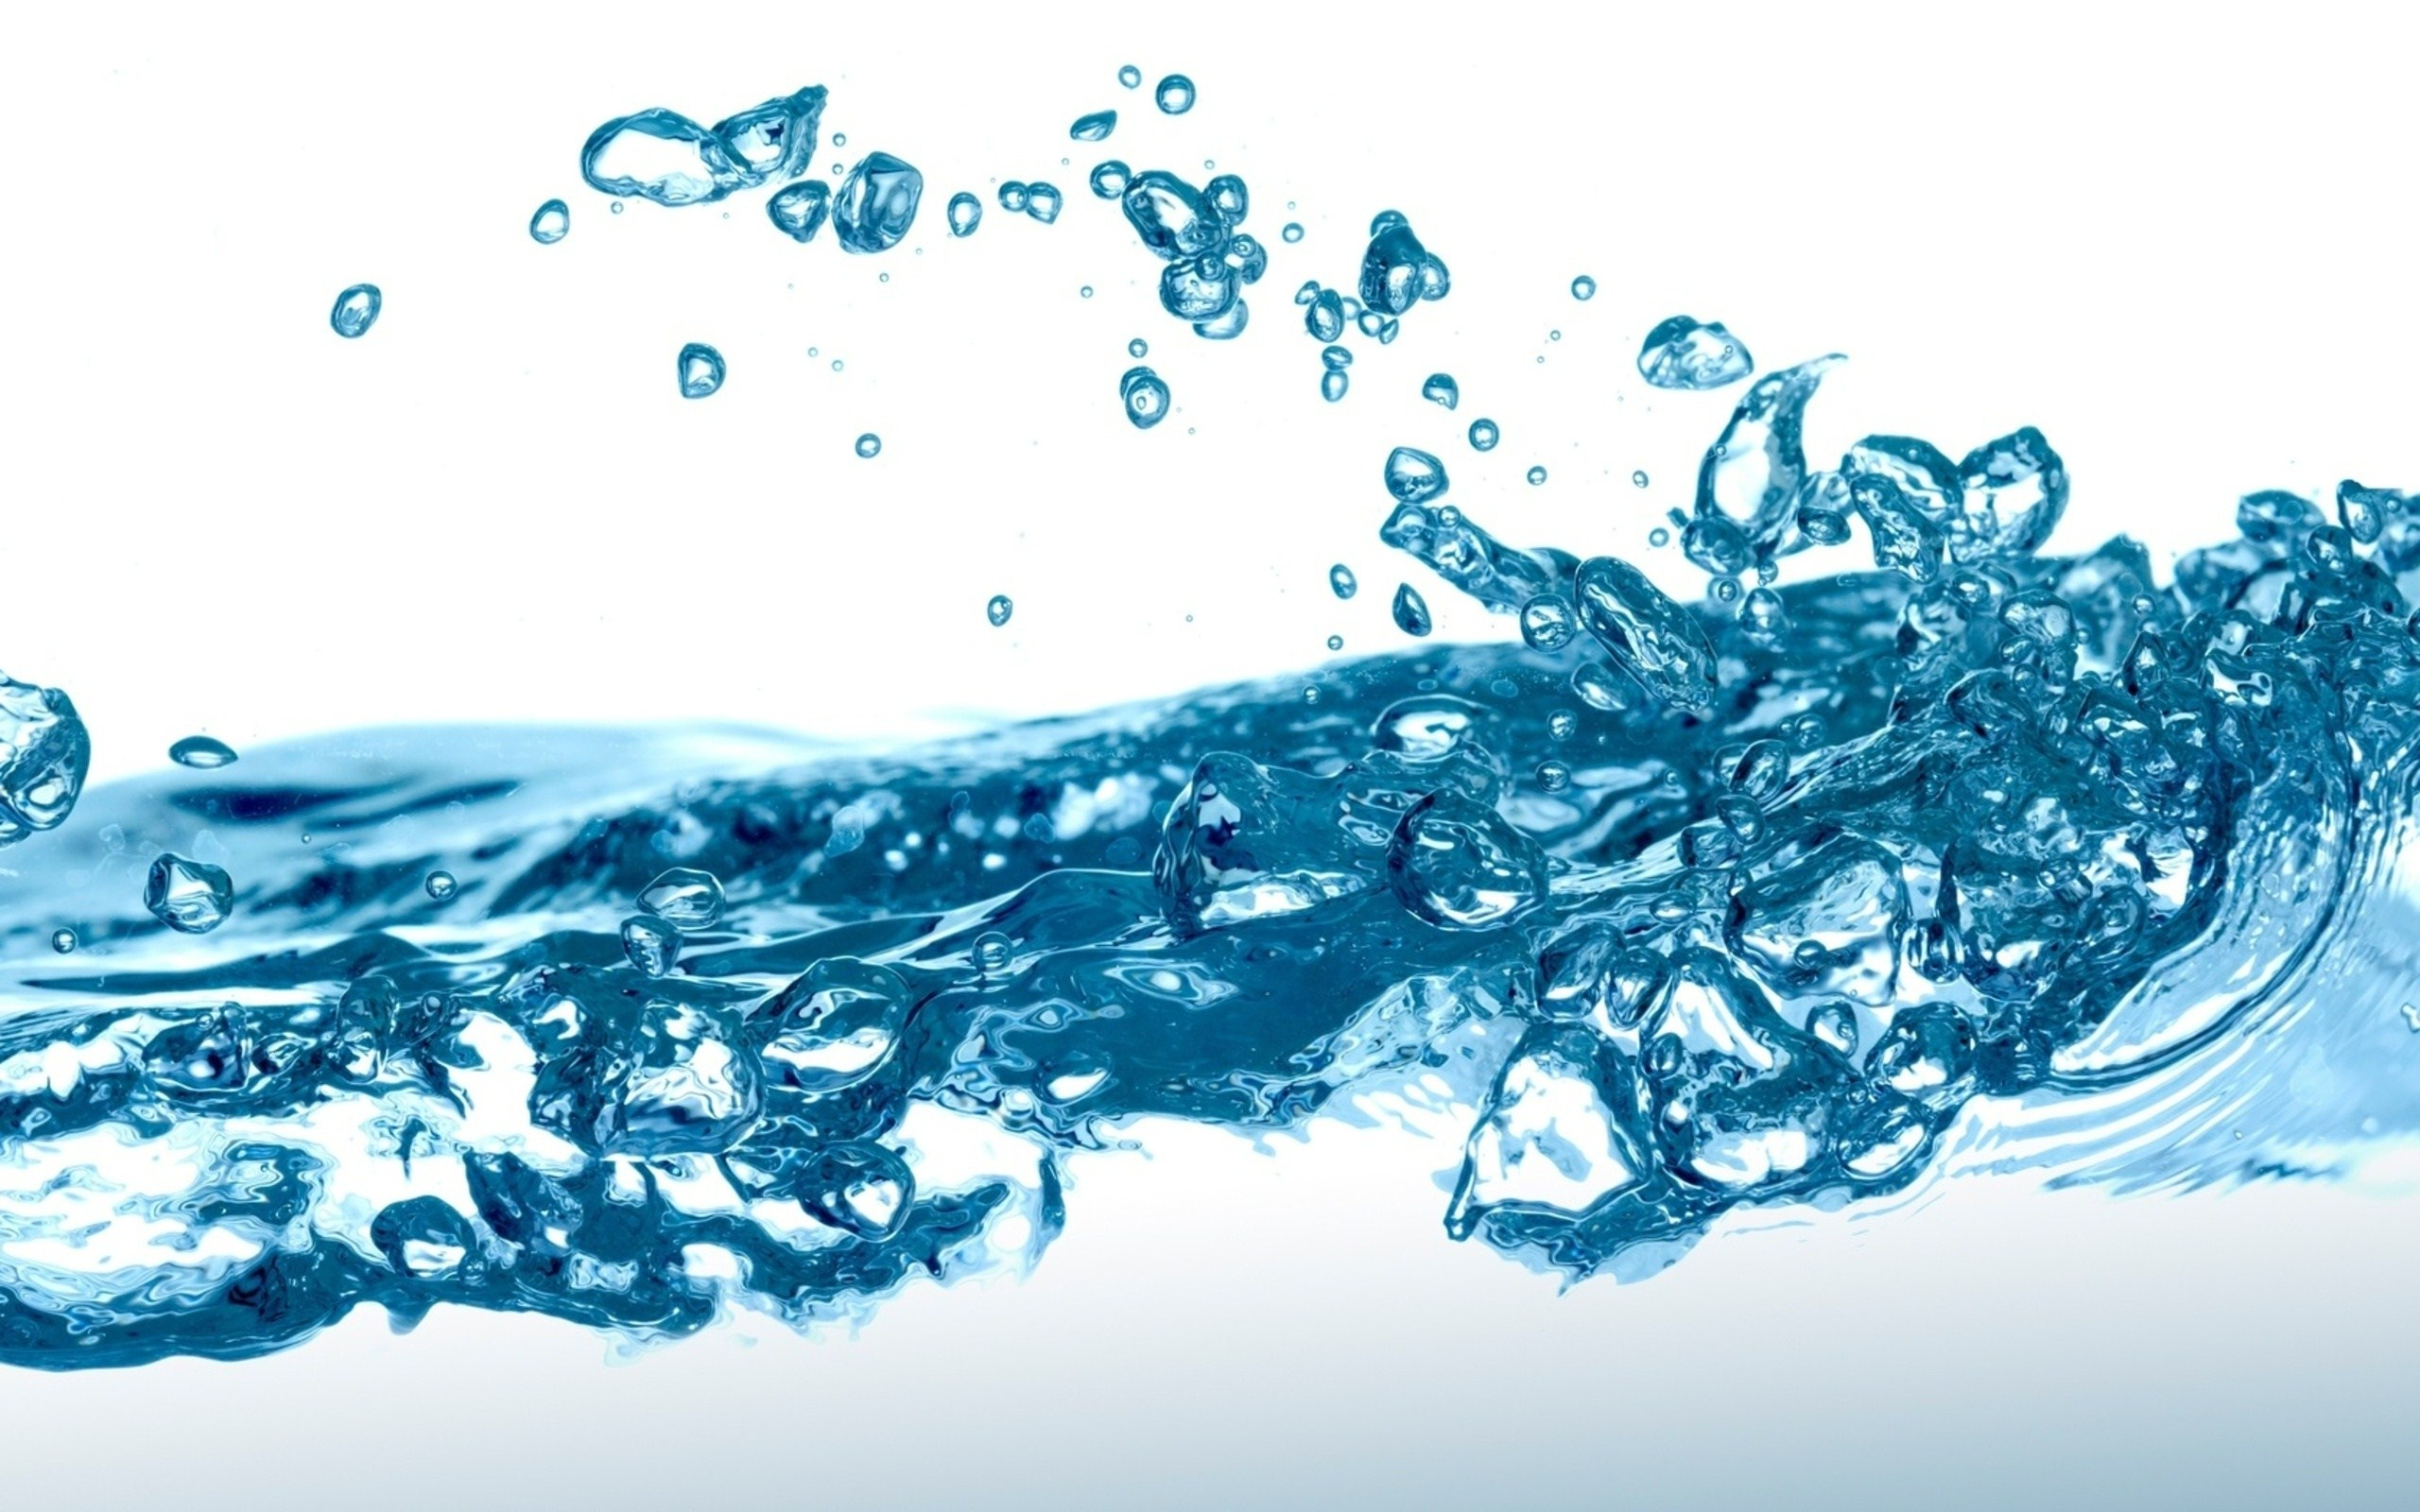
\includegraphics[width=\paperwidth]{figs/background}}
  \begin{frame}
    \maketitle
    \begin{center}
      Dr. David Roundy, Department of Physics
      \vspace{1.5in}
    \end{center}

  \end{frame}
}

% slides 2,3: background / application

\begin{frame}
  \frametitle{Long Term Goals}
  In addition to wanting a better understanding of water, many important things happen in contact with water
  \begin{itemize}
  \item Rust
  \item Surfactants, e.g. soap
  \item Acid-base reactions
  \item Cells
  \end{itemize}\vspace{.5in}
  Final goal: to efficiently compute properties of systems involving water
\end{frame}

\begin{frame}
  \frametitle{Goals of this Project}
  \begin{itemize}\itemsep2ex
  \item Theory for liquids not well understood
  \item Almost exclusively based on hard spheres
    \begin{itemize}
    \item Hard sphere fluid: Spherical particles with no interaction except that they cannot overlap
    \end{itemize}
  \item Spheres want 12 neighbors, water molecules want 4
  \end{itemize}\vspace{.25in}
  Explore the properties of various hard polyhedra fluids, in particular truncated tetrahedra

  \begin{figure}[b]
    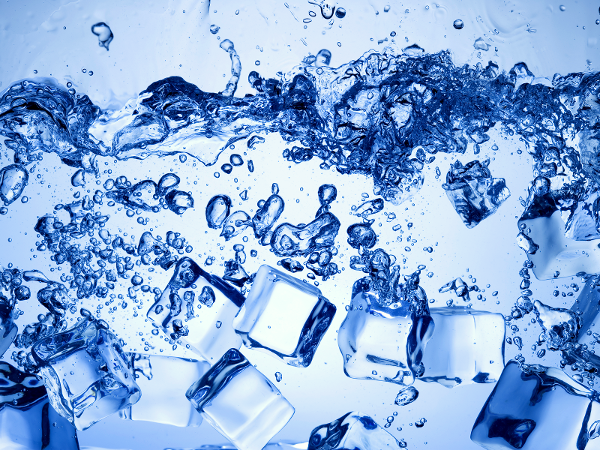
\includegraphics[width=60mm]{figs/ice-water.png}
  \end{figure}

\end{frame}

% slide 4: ice structure image
\begin{frame}
  \frametitle{Why Truncated Tetrahedra}
  \begin{columns}[T,totalwidth=\textwidth]
    \column{.2\linewidth}
    \begin{figure}[h]
      \includegraphics[width=30mm]{figs/tet-0}\\
      \includegraphics[width=30mm]{figs/tet-1}\\
      \includegraphics[width=30mm]{figs/tet-2}
    \end{figure}
    \column{.8\linewidth}
    \begin{overprint}
      \begin{figure}[t]
        \centering
        \includegraphics<1>[width=90mm]{figs/ice-structure-0}
        \includegraphics<2>[width=90mm]{figs/ice-structure-1}
        \includegraphics<3>[width=90mm]{figs/ice-structure-2}
        \includegraphics<4>[width=90mm]{figs/ice-structure-3}
        \includegraphics<5>[width=90mm]{figs/ice-structure-4}
      \end{figure}
    \end{overprint}
  \end{columns}
\end{frame}

% slide 5: mc, explanation

\begin{frame}
  \frametitle{Simple 2d Fluid Between Parallel Walls}
  \begin{columns}[T,totalwidth=\textwidth]
    \column{.65\linewidth}
  \begin{figure}[h]
    \centering
    \animategraphics[width=\columnwidth]{.6}{anim/mc-slow-}{000}{029}
  \end{figure}
  \column{.35\linewidth}
  Monte Carlo Method:
  \begin{itemize}
  \item Average of many configurations
  \item Move and rotate to get from one configuration to the next
  \item Reject any moves that overlap
  \end{itemize}
  \end{columns}
\end{frame}

% slide 6: mc example with density / angles
\begin{frame}
  \frametitle{Hard Triangle Fluid Between Parallel Walls}
  \begin{figure}[h]
    \centering
    \animategraphics[width=100mm,final]{.6}{anim/mc100-0.50-}{000}{029}
  \end{figure}
\end{frame}

% slides 7-8: similar to slide 6, but with 3d cubes, fluid and then solid
\begin{frame}
  \frametitle{Hard Cube Fluid Between Parallel Walls}
  \begin{figure}[h]
    \centering
    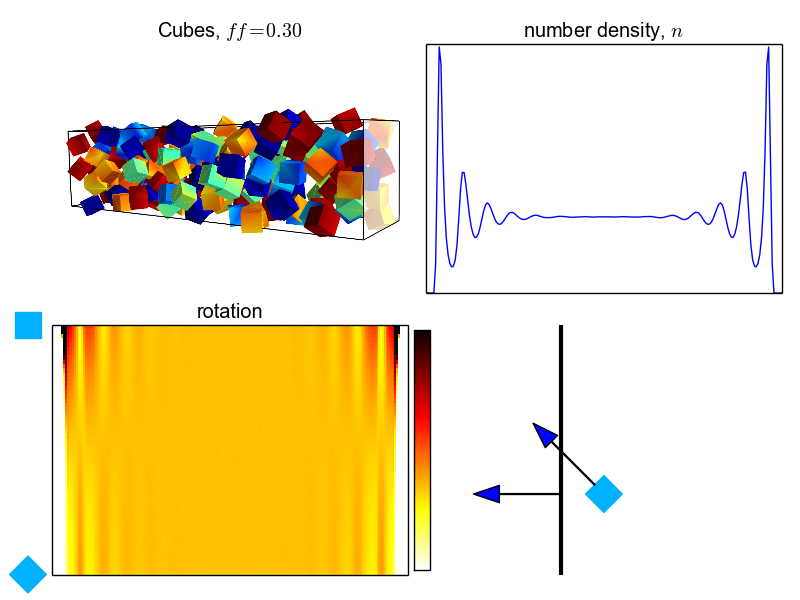
\includegraphics[width=100mm]{figs/cube-density-30}
  \end{figure}
\end{frame}

\begin{frame}
  \frametitle{Hard Cube Solid Between Parallel Walls}
  \begin{figure}[h]
    \centering
    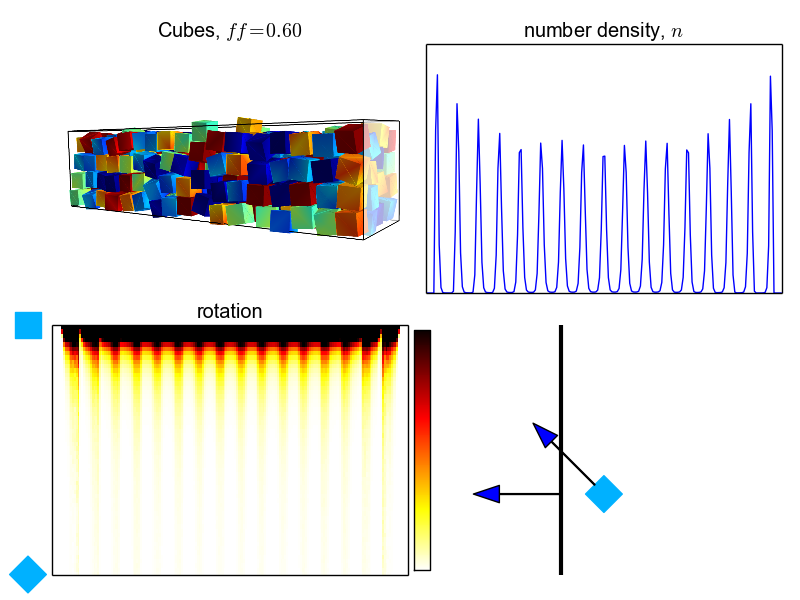
\includegraphics[width=100mm]{figs/cube-density-60}
  \end{figure}
\end{frame}

\begin{frame}
  \frametitle{Fluid and Solid Truncated Tetrahedra}
  \begin{figure}[h]
    \centering
\animategraphics[width=55mm,autoplay,loop,final]{1}{../../papers/polyhedra/figs/anim/periodic-0.42-truncated_tetrahedron-216-}{0}{9} \animategraphics[width=55mm,autoplay,loop,final]{1}{../../papers/polyhedra/figs/anim/periodic-0.71-truncated_tetrahedron-216-}{0}{9}
  \end{figure}
\end{frame}

% slide 10: conclusion
\begin{frame}
  \frametitle{Conclusions}
  \begin{itemize}\itemsep2ex
  \item Wrote a program for simulating hard polyhedra
  \item Constructed ice with truncated tetrahedra
  \item Observed the solid and fluid phases of truncated tetrahedra
  \item Future work:
    \begin{itemize}
    \item Explore correlations between truncated tetrahedra
    \item Examine angular dependence in truncated tetrahedra
    \item Observe phase transitions in truncated tetrahedra
    \end{itemize}

  \end{itemize}
\end{frame}

\begin{frame}
  \frametitle{Acknowledgements}
  \begin{itemize}\itemsep2ex
  \item Undergraduate Research, Innovation, Scholarship, \& Creativity (URISC)
  \item Dr. David Roundy
  \item Research Group: Jeff Schulte, Eric Krebs, Rene Zeto, Sam Loomis, Dan Roth, Daniel Gluck
  \end{itemize}
\end{frame}

\end{document}
